%%%%%%%%%%%%%%%%%%%%%%%%%%%%%%%%%%%%%%%%%%%%%%%%%%%%%%%%%%%%%%%%%%%%%%
%     File: ExtendedAbstract_imple.tex                               %
%     Tex Master: ExtendedAbstract.tex                               %
%%%%%%%%%%%%%%%%%%%%%%%%%%%%%%%%%%%%%%%%%%%%%%%%%%%%%%%%%%%%%%%%%%%%%%

\section{Aerial-D}
\label{sec:approach}

Existing referring expression datasets primarily focus on natural scene imagery, leaving a significant gap in aerial domain applications where objects exhibit different characteristics, spatial relationships, and visual properties. To address this limitation, we present Aerial-D, a comprehensive referring expression dataset specifically designed for aerial imagery segmentation tasks. Our approach transforms existing aerial segmentation datasets into rich referring expression resources through systematic rule-based generation followed by large language model enhancement.

The construction of Aerial-D builds upon two complementary source datasets with fundamentally different annotation paradigms. The iSAID dataset provides high-resolution aerial images with instance segmentation annotations across 15 object categories including ships, vehicles, planes, buildings, and infrastructure elements. In contrast, the LoveDA dataset offers semantic segmentation data capturing land cover patterns such as buildings, water bodies, agricultural areas, and forests. These datasets ensure comprehensive coverage of both discrete objects and continuous landscape features commonly encountered in aerial imagery.

Our preprocessing pipeline extracts 480×480 patches from both source datasets using sliding window approaches with controlled overlap. For iSAID data, we preserve existing instance annotations while handling boundary objects through intersection ratio analysis. For LoveDA data, we apply connected components analysis to convert semantic segmentation masks into individual instances for building and water categories, while treating other land cover types as unified semantic classes. This dual approach balances instance-level detail with semantic coverage across diverse aerial content.

\subsection{Rule-Based Expression Generation}

The foundation of our dataset construction relies on systematic rule-based generation that analyzes spatial, visual, and relational properties of objects within aerial imagery. Our pipeline transforms basic segmentation annotations into rich referring expressions through comprehensive feature extraction and linguistic synthesis.

\begin{figure}[H]
\centering
\begin{minipage}{0.5\textwidth}
\centering
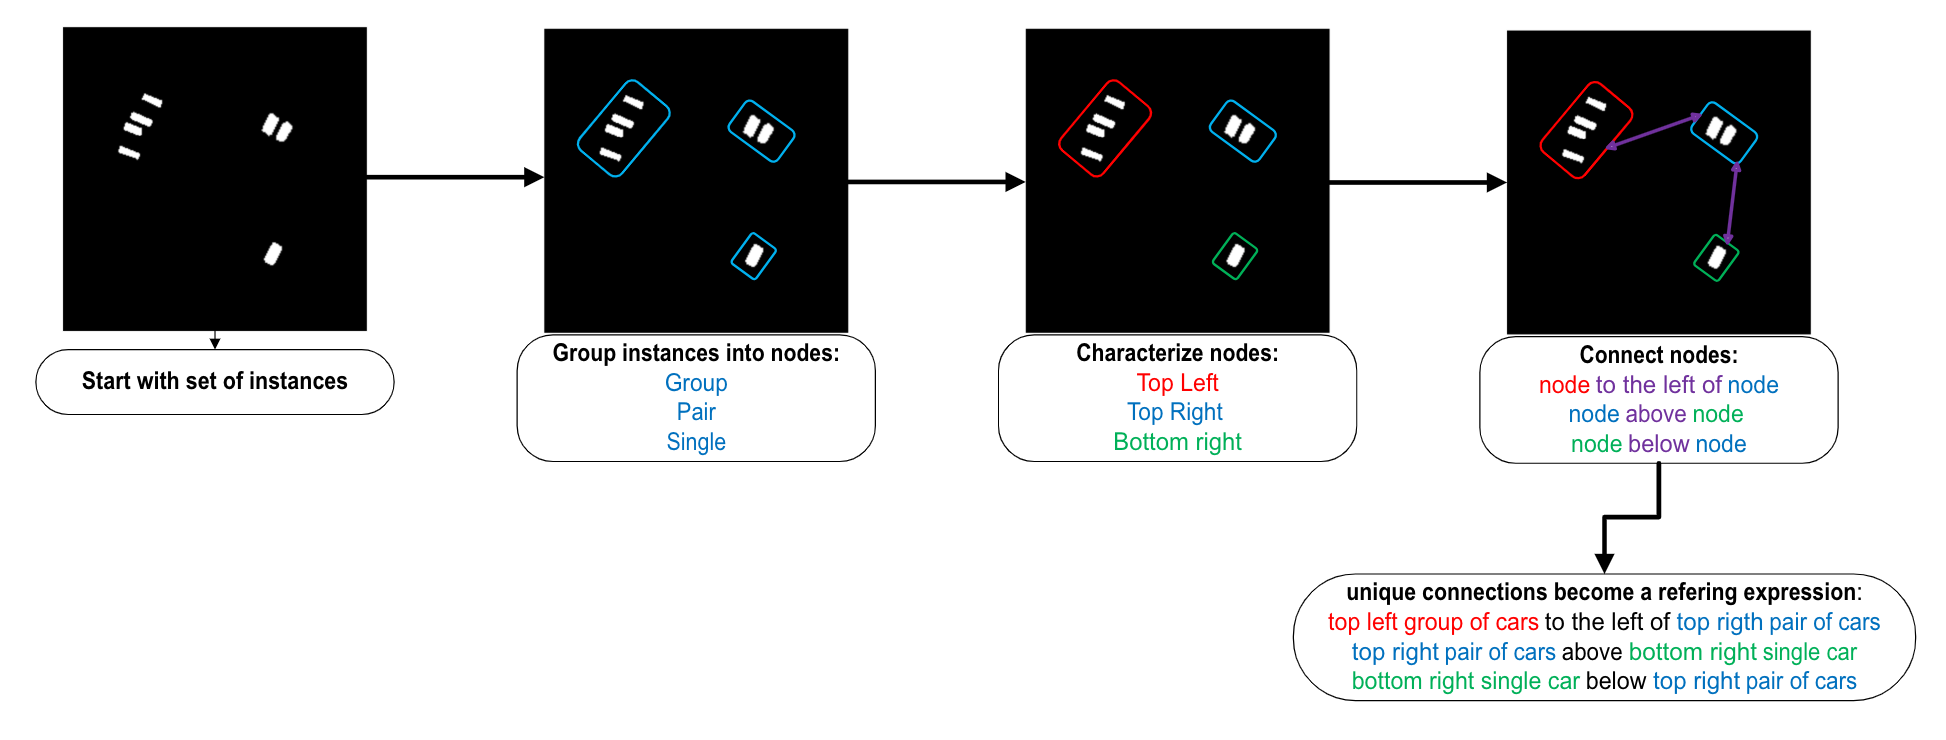
\includegraphics[width=0.7\textwidth]{./images/rule_based_generation.png}
\end{minipage}%
\begin{minipage}{0.5\textwidth}
\centering
\hspace{-1cm}
\raisebox{-0.3\height}{%
\resizebox{\textwidth}{!}{%
\footnotesize
\begin{tabular}{@{}ll@{}}
\toprule
\textbf{Rule Type} & \textbf{Example Instance} \\
\midrule
Category & "plane" \\
Grid Position & "in the top right" \\
Extreme Position & None \\
Color Classification & "light" \\
Directional Relations & "to the bottom right of a plane" \\
& "to the top right of a plane" \\
\midrule
\multicolumn{2}{l}{\textbf{Final Expressions}} \\
\multicolumn{2}{l}{"the plane in the top right"} \\
\multicolumn{2}{l}{"the light plane in the top right"} \\
\multicolumn{2}{l}{"the plane in the top right to the bottom right of a plane"} \\
\multicolumn{2}{l}{"the light plane in the top right to the bottom right of a plane"} \\
\multicolumn{2}{l}{"the plane in the top right to the top right of a plane"} \\
\multicolumn{2}{l}{"the light plane in the top right to the top right of a plane"} \\
\bottomrule
\end{tabular}%
}%
}
\end{minipage}
\caption{Example of rule generation for a single instance. The highlighted plane in the top right section demonstrates how the system assigns spatial, visual, and relational rules that will later be combined into referring expressions.}
\label{fig:rule_example}
\end{figure}

Each 480×480 patch undergoes spatial analysis through grid partitioning into nine distinct regions, establishing fundamental positional references such as "top left", "center", and "bottom right". To handle objects positioned near boundaries between regions, we implement borderline detection that assigns multiple valid position labels when objects fall within boundary zones. This ensures robust expression coverage while maintaining spatial precision.

Visual feature extraction focuses on color classification within HSV color space, distinguishing between achromatic properties (light and dark variations) and chromatic characteristics across distinct hue ranges. The system requires statistical dominance thresholds to ensure reliable color assignment, avoiding ambiguous classifications that could mislead referring expressions. However, we selectively filter chromatic references for certain categories like buildings and water, which typically exhibit complex multi-hue patterns unsuitable for color-based discrimination.

Spatial relationship analysis establishes connections between nearby objects through angle-based directional systems. The system calculates relative positioning between object pairs using dynamic distance thresholds that account for object scale, ensuring meaningful proximity relationships while preventing spurious long-distance connections. This enables expressions that describe objects relative to nearby instances, such as "the ship to the left of the harbor".

To handle scenarios with multiple similar objects, we implement clustering-based group formation that identifies spatially proximate instances of the same category. The clustering approach utilizes minimum bounding box distances rather than centroid distances, providing more accurate spatial proximity assessment. This enables collective referring expressions for groups of similar objects while maintaining individual instance coverage.

The expression synthesis process combines all extracted features through systematic template application, generating linguistic descriptions ranging from simple category references to complex multi-attribute formulations. However, comprehensive generation inevitably creates conflicting expressions where identical phrases refer to multiple different objects. We address this ambiguity through strict uniqueness filtering that eliminates all non-unique expressions, ensuring every remaining phrase uniquely identifies a single target within the dataset.

\begin{figure}[H]
\centering
\begin{minipage}{0.5\textwidth}
\centering
\includegraphics[width=0.7\textwidth]{./images/filter_unique.png}
\end{minipage}%
\begin{minipage}{0.5\textwidth}
\centering
\hspace{-1cm}
\raisebox{-0.3\height}{%
\resizebox{\textwidth}{!}{%
\footnotesize
\begin{tabular}{@{}ll@{}}
\toprule
\textbf{Expression} & \textbf{Status} \\
\midrule
\multicolumn{2}{l}{\textbf{Object 1 (Light Vehicle)}} \\
\midrule
"the small vehicle in the top right" & \textcolor{red}{Filtered} \\
"the topmost small vehicle" & \textcolor{green!70!black}{Kept} \\
"the light small vehicle in the top right" & \textcolor{green!70!black}{Kept} \\
"the light topmost small vehicle" & \textcolor{green!70!black}{Kept} \\
"the small vehicle in the top right above a small vehicle" & \textcolor{green!70!black}{Kept} \\
\midrule
\multicolumn{2}{l}{\textbf{Object 2 (Dark Vehicle)}} \\
\midrule
"the small vehicle in the top right" & \textcolor{red}{Filtered} \\
"the dark small vehicle in the top right" & \textcolor{green!70!black}{Kept} \\
"the small vehicle in the top right below a small vehicle" & \textcolor{green!70!black}{Kept} \\
\bottomrule
\end{tabular}%
}%
}
\end{minipage}
\caption{Example of expression uniqueness filtering. When two objects share similar attributes, conflicting expressions like "the small vehicle in the top right" are filtered out, while unique expressions that distinguish between objects are retained.}
\label{fig:filter_unique_example}
\end{figure}

\subsection{LLM Expression Generation}

While rule-based generation provides systematic coverage of spatial and visual attributes, the resulting expressions suffer from limited linguistic variation and restricted contextual detail. Rule-based templates produce linguistically constrained expressions that lack the natural language diversity essential for robust model training. Additionally, these expressions are confined to predefined object classes and cannot reference contextual elements that could provide richer spatial descriptions.

To address these limitations, we employ large language model enhancement through two primary mechanisms. Language enhancement diversifies the linguistic patterns beyond simple templates, generating varied phrasings and vocabulary while maintaining semantic accuracy. Visual enhancement incorporates detailed descriptions of contextual objects and environmental features that extend beyond the original dataset categories, enabling expressions that reference nearby roads, vegetation, and architectural elements not captured in the source annotations.

\begin{figure}[H]
\centering
\begin{minipage}{0.5\textwidth}
\centering
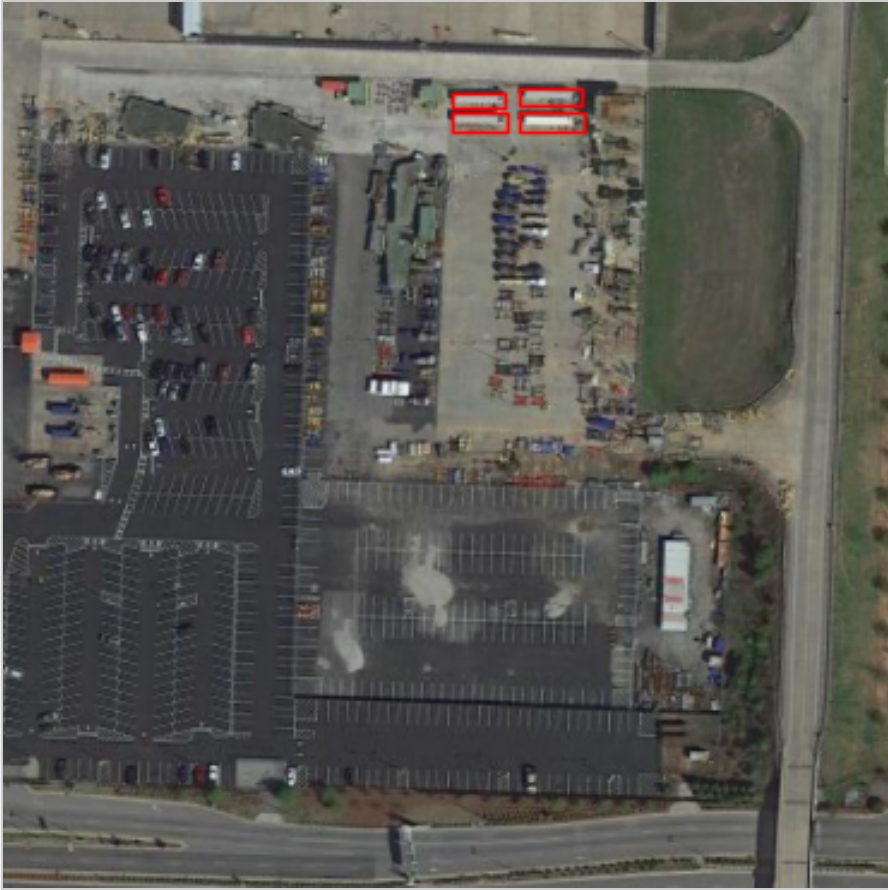
\includegraphics[width=0.7\textwidth]{./images/example_group.png}
\end{minipage}%
\begin{minipage}{0.5\textwidth}
\centering
\hspace{-1cm}
\raisebox{-0.3\height}{%
\footnotesize
\begin{tabular}{@{}p{2cm}p{5cm}@{}}
\toprule
\textbf{Expression Type} & \textbf{Example} \\
\midrule
Original & the group of 4 large vehicles in the top center \\
\midrule
Enhanced & the cluster of four big vehicles near the upper middle \\
\midrule
Unique & the four large vehicles lined up side by side just below the pale paved strip at the very top middle \\
\midrule
Unique & the set of four big vehicles parked in a single row in the upper center beside the grassy area to the right \\
\bottomrule
\end{tabular}%
}
\end{minipage}
\caption{Example of LLM enhancement process showing original aerial image with group of four large vehicles (left) and corresponding expression enhancements (right).}
\label{fig:llm_enhancement_example}
\end{figure}

However, applying production-grade language models directly to our dataset presents significant computational challenges. The rule-based generation produces hundreds of thousands of expressions requiring LLM processing, creating scale that would be prohibitively expensive using premium APIs. Processing the complete dataset through high-quality proprietary models would require substantial financial resources and extensive processing time.

We implement knowledge distillation to transfer capabilities from large proprietary models to smaller, deployable alternatives. Our distillation pipeline begins by processing a carefully selected subset of 500 representative samples through OpenAI's o3 model, leveraging high-quality production capabilities to generate optimal expression enhancements. These outputs capture desired enhancement patterns including language variation, visual detail incorporation, and contextual spatial references.

The collected high-quality outputs serve as training data for fine-tuning Gemma3-12B, an open-source multimodal model with accessible weights. Through QLora fine-tuning techniques, we transfer the enhancement knowledge demonstrated by o3 into the more compact Gemma3 architecture. This fine-tuned model enables local deployment using vLLM inference on standard GPU hardware to process the entire dataset.

The distillation approach transforms costly premium API processing into manageable local inference operations. The fine-tuned Gemma3 model generates millions of enhanced expressions across the complete dataset while maintaining enhancement quality comparable to the original o3 outputs. This scalable solution enables comprehensive dataset enhancement without the computational and financial constraints of direct premium model application.

\begin{figure}[H]
\centering
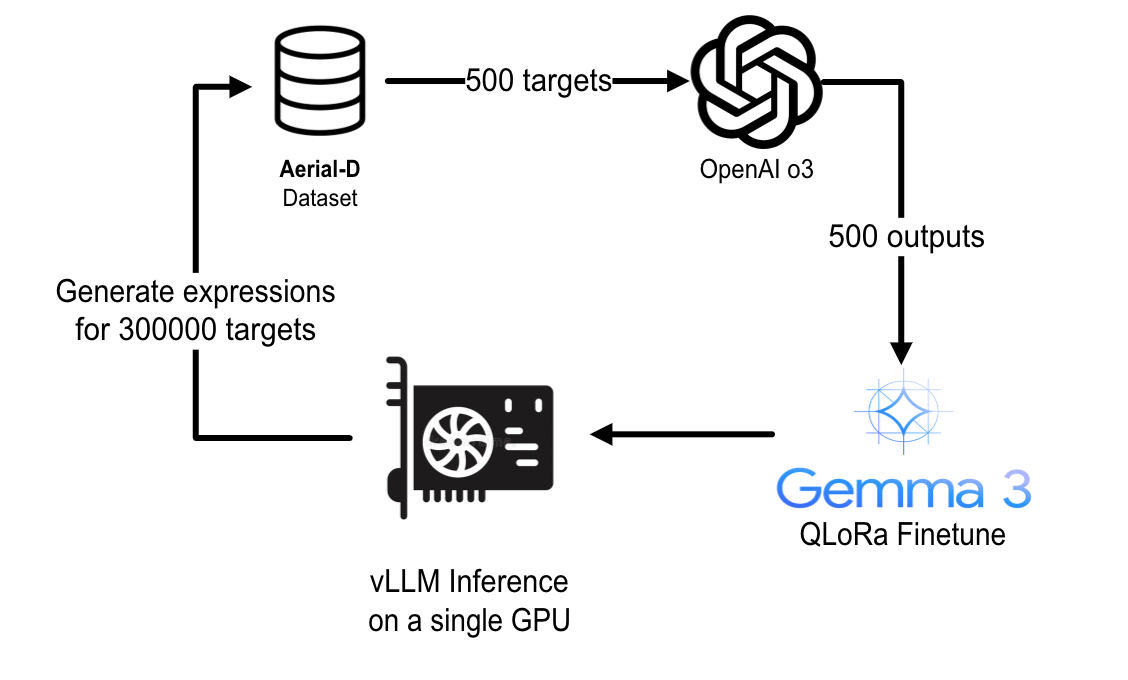
\includegraphics[width=0.6\textwidth]{./images/distillation.png}
\caption{Knowledge distillation pipeline for scalable LLM enhancement. A small sample of 500 expressions is processed through OpenAI's O3 model to generate high-quality training targets, which are then used to fine-tune Gemma3 12B via QLora. The fine-tuned model enables cost-effective local inference to enhance the full dataset of 300,000 expressions using vLLM on a single GPU.}
\label{fig:llm_distillation}
\end{figure}
\end{figure>

The completed Aerial-D dataset represents a significant advancement in aerial referring expression resources. The final dataset contains 37,288 patches with 259,709 annotated samples generating over 1.5 million total expressions. The systematic generation maintains balanced distribution between individual objects (128,715 instances with 889,354 expressions) and groups (130,994 groups with 633,169 expressions), averaging approximately 7 expressions per individual object and 5 expressions per group. LLM enhancement successfully tripled the original dataset size, contributing nearly equal numbers of language variations (496,895) and unique visual detail expressions (519,434) to the original 506,194 rule-based expressions. This comprehensive coverage across object categories, spatial relationships, and linguistic diversity provides essential training resources for robust referring segmentation model development.

